\section{Presentation Layer Design}

The application's user interface is built on a single main window, in which the application's main content is only loaded after a user successfully authenticates. The entire user interface is built in a hierarchical structure, in which the main screen contains all the sub-components specific of each functionality, as the following figure shows. Each static UI component is defined with its own FXML file, the detailed explanation of the structure's functionality comes in the next chapter.

\begin{figure}[htbp]
\centering
\begin{minipage}{0.5\textwidth}
\dirtree{%
.1 resources/.
.2 popups/.
.3 assignments/.
.4 popup\_create\_assignment.fxml.
.3 expenses/.
.4 popup\_create\_expense.fxml.
.4 popup\_you\_owe.fxml.
.4 popup\_you\_are\_owed.fxml.
.4 popup\_settle\_debt.fxml.
.3 household/.
.4 popup\_create\_chore.fxml.
.4 popup\_manage\_members.fxml.
.4 popup\_invite\_member.fxml.
.4 popup\_chores\_list.fxml.
.4 popup\_shopping\_lists.fxml.
.4 popup\_list\_details.fxml.
.4 popup\_create\_household.fxml.
.3 user/.
.3 popup\_confirm.fxml.
.2 tabs/.
.3 household\_tab\_wrapper/.
.4 tab\_household.fxml.
.4 tab\_no\_household.fxml.
.3 tab\_assignments.fxml.
.3 tab\_expenses.fxml.
.3 tab\_user.fxml.
.2 auth.fxml.
.2 main.fxml.
}
\end{minipage}
\caption{Frontend FXML Structure}
\end{figure}

As the directory structure shows, the authentication screen is completely separated from the real application area, and the main file contains all of the other sub-components within it, more precisely they are loaded in a specific component of that file which will serve as the main content container. The user interface makes use of popups to display and allow interaction with the application's main functionalities. 

\begin{figure}
    \centering
    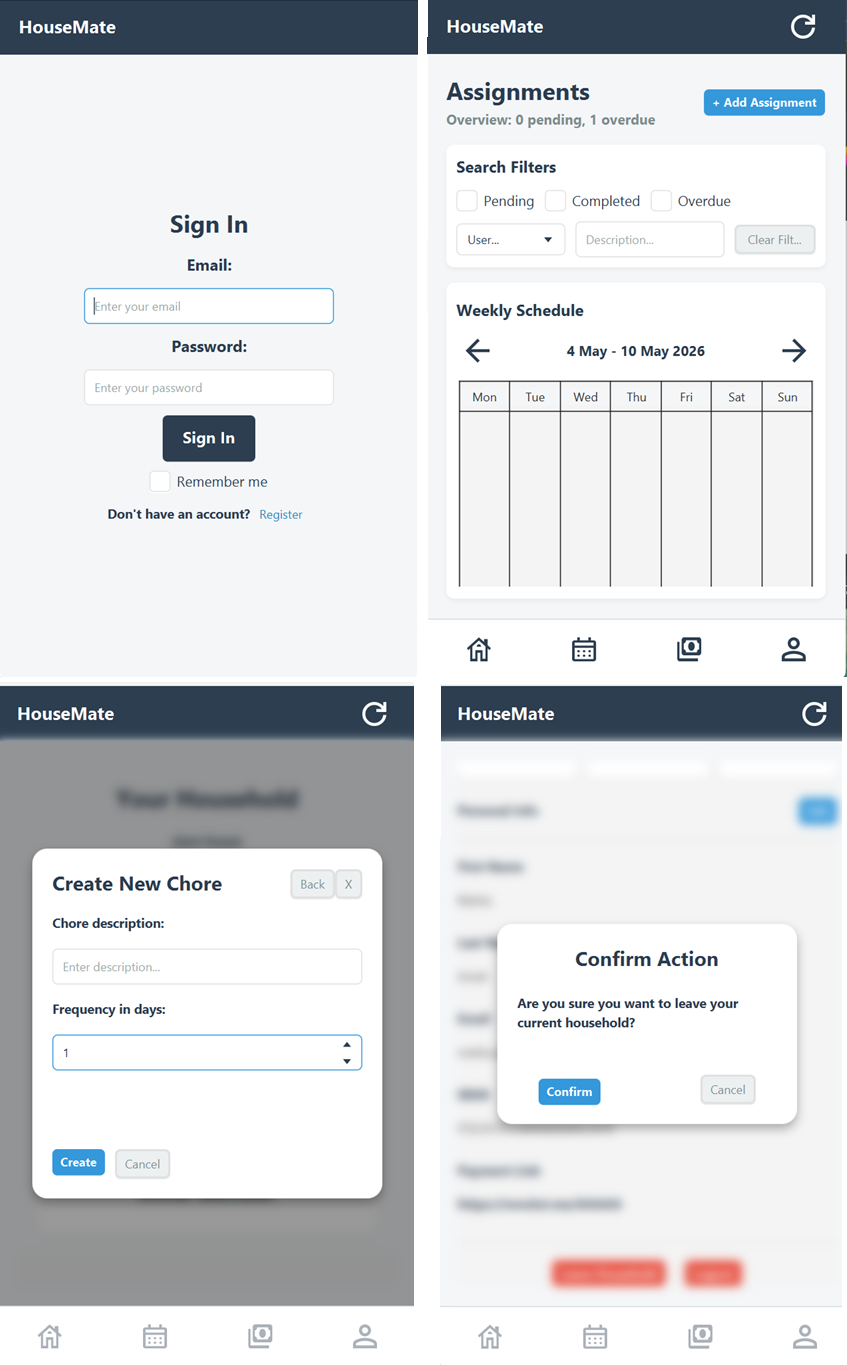
\includegraphics[width=0.8\linewidth]{images/complete_ui_screenshot..png}
    \caption{Examples of the user interface's appearance and structure}
\end{figure}

The images make clear how the authentication screen is completely separate from the rest of the client, how the main application is composed of the four tabs (Household, Assignments, Expenses, User) and how each tab contains its own popups for specific functionalities.




\section{Frontend-Backend Communication}

\subsection{Performing HTTP Requests}

The application's client module is able to communicate with the backend by performing HTTP requests to the endpoints it exposes. This responsibility is assigned to the \texttt{ClientService} classes, of which there is one for each principal domain model entity and which expose simple Java methods to the UI handling code, and act as bridges between the Java objects required by JavaFX to handle data and the JSON payloads that the backend module responds to calls with. All the client services are composed with a base helper class, \texttt{HttpRestClient}, whose responsibilities are performing that Java-JSON translation (serialization-deserialization) with the \texttt{ObjectMapper} class from the \texttt{Jackson} dependency and actually sending the HTTP request, using the native Java module \texttt{java.net.http.HttpClient} and handling all the specific exceptions that the methods of these classes can throw. Using these helper methods, the ones in the client service classes become extremely simple:
\newline
\begin{lstlisting}[language=Java, caption=Example of an HTTP request performing method in the client services (UserClientService)]
public UserResponseDTO updateCurrentUser(UserUpdateRequestDTO requestDTO) {
    String requestBody = httpRestClient.serializeDTO(requestDTO);

    HttpRequest request = HttpRequest.newBuilder()
            .uri(URI.create(BASE_URL + "/api/users/me"))
            .header("Content-Type", "application/json")
            .header("Accept", "application/json")
            .header("Authorization", httpRestClient.buildAuthHeader())
        .method("PATCH", HttpRequest.BodyPublishers.ofString(requestBody))
            .build();

    HttpResponse<String> response = httpRestClient.sendRequest(request);

    if (response.statusCode() == 200) {
        return httpRestClient.deserializeDTO(response.body(), UserResponseDTO.class);
    }

    throw new RuntimeException(
            "Failed to update current user. Server responded with status code: " + response.statusCode() + " and message: " + response.body()
    );
}
\end{lstlisting}

It is noticeable how every request includes a header with the user's JWT to authenticate itself and pass through the security layers.


\subsection{Storing Key Information}
The application is able to maintain in the client's system some useful data, to avoid clogging the server with multiple backend calls for the same purpose: this is implemented by the \texttt{SessionManager}, \texttt{AppServices}, and \texttt{JwtPersistanceHandler classes}, which respectively have the following responsibilities:
\begin{itemize}
    \item \texttt{SessionManager:} contains instances of Response DTOs related to the currently logged user, its household and its members: this data is updated when a refresh is performed, and is used on many different backend calls. Not including this would require the client to perform an additional request for almost every functionality, effectively doubling the load on the server.
    \item \texttt{AppServices:} serves as a wrapper class: it contains an instance of each different client service, as well as the SessionManager instance. This is almost required to make the injection of all the dependencies down the Controller classes possible: not using this class would add tens of lines of boilerplate code to every load of a different page.
    \item \texttt{JwtPersistanceHandler:} used to implement the "Remember Me" functionality. Since a user can authenticate itself with a valid JWT if the option to do so is chosen, this class relies on the Java native \texttt{java.util.prefs.Preferences}, which safely stores the token (received from the login endpoint) in a system registry and is able to retrieve it and attempt to use it to skip the email-and-password login step. If the token saved in the system expires or becomes no longer valid in any way, the application falls back to the standard login screen.
\end{itemize}


\section{UI/UX Functionalities}

\subsection{FXML Page Building and Loading}
The core building block of all the application's user interface are the static pages built with FXML files. These files consist of a composition of JavaFX components, which can generally be referred to as nodes, nested into each other to allow the construction of organized and well-defined layouts. Here follows, as an example, part of the main page's code:\clearpage

\begin{lstlisting}[language=XML, caption=Core structure of the client's main window]
<BorderPane prefHeight="750.0" prefWidth="420.0" styleClass="root" xmlns="http://javafx.com/javafx/21" xmlns:fx="http://javafx.com/fxml/1" fx:controller="com.housemate.client.controllers.MainController">
    <top>
        <!--Logo and "Refresh" button-->
    </top>

    <center>
        <StackPane fx:id="outerContainer">
            <StackPane fx:id="mainContentContainer"/>
            <StackPane fx:id="popupLayer" mouseTransparent="true"/>
            <StackPane fx:id = "confirmPopupLayer" mouseTransparent="true"/>
        </StackPane>
    </center>

    <bottom>
        <HBox alignment="CENTER" prefHeight="60.0" styleClass="nav-bar" BorderPane.alignment="CENTER">
            <Button fx:id="btnNavH" maxWidth="Infinity" prefHeight="60.0" styleClass="nav-button-active" HBox.hgrow="ALWAYS">
                <graphic>
                    <Region styleClass="base-icon, household-nav-button"/>
                </graphic>
            </Button>
            <!--Three more exactly equal buttons for the other tabs-->
        </HBox>
    </bottom>

</BorderPane>
\end{lstlisting}

As the first statement of the example shows, each file is linked to its own Controller Java class with the \texttt{fx:controller} attribute within the root node. These classes are responsible for handling the interactions between the user and the interface elements, performing calls to the client services and visualizing incoming data from the backend.
\newline

The Controller hierarchy is exactly the same as the fxml files one, since they are in a 1:1 relationship.

\begin{lstlisting}[language=Java, caption=Code to load a FXML file (from the MainController class)]
FXMLLoader loaderAssignments = new FXMLLoader(getClass().getResource("/com/housemate/client/tabs/tab_assignments.fxml"));
loaderAssignments.setControllerFactory(clazz -> new TabAssignmentsController(this.services, this));
tabAssignments = loaderAssignments.load();
tabAssignmentsController = loaderAssignments.getController();
\end{lstlisting}

All the loaders have to use the \texttt{setControllerFactory} method to allow the injection of the \texttt{AppServices} and other required dependencies to the corresponding Controllers.

\subsection{Hierarchical Structure of the Controllers}

\begin{figure}[H]
\centering
\begin{minipage}{0.5\textwidth}
\dirtree{%
.1 controllers/.
.2 AuthScreenController.java.
.2 MainController.java/.
.3 PopupConfirmActionController.java.
.3 HouseholdTabWrapperController.java/.
.4 TabHouseholdController.java/.
.5 PopupChoresList.java.
.5 PopupCreateChoreController.java.
.5 PopupCreateListController.java.
.5 PopupInviteMemberController.java.
.5 PopupListDetailsController.java.
.5 PopupManageMembersController.java.
.5 PopupShoppingListsController.java.
.4 TabNoHouseholdController.java/.
.5 PopupCreateHouseholdController.java.
.5 PopupJoinHouseholdController.java.
.3 TabAssignmentsController.java/.
.4 PopupCreateAssignmentsController.java.
.3 TabExpensesController.java/.
.4 PopupCreateExpenseController.java.
.4 PopupSettleDebtController.java.
.4 PopupYouAreOwedController.java.
.4 PopupYouOweController.java.
}
\end{minipage}
\caption{Complete structure of the Controller hierarchy}
\end{figure}

As the previous code snippet and the structure diagram showed, when the \texttt{MainController} loads the FXML files relative to the four main application tabs, it passes itself (\texttt{this}) down to their Controllers. This has been repeated in the following steps, such that the tabs Controllers pass down the \texttt{MainController} reference to those of the popups they load. This structure has been chosen to allow the main controller to be the only responsible for showing graphical elements to the user: whenever any Controller wants a popup to be opened, a different tab to be displayed or a success/error message to be displayed, all they have to do is call the \texttt{MainController}'s corresponding methods.

This implementation allows for both paths of the hierarchy to be taken: when a button within a tab is clicked, the corresponding controller can call both the \texttt{MainController} to open a popup and call the popup's controller itself to perform some actions, which is usually the backend call to fetch the information specific to that popup. 

\subsection{Application Launch}
All JavaFX applications are required to have their entry point defined by a class which extends \texttt{javafx.Application}. The main method of the program has to call the static method \texttt{Application.launch()}: JavaFX then automatically calls the \texttt{start} method, which has to be overridden in the entry point class. Here is part of HouseMate's client launcher class:
\clearpage

\begin{lstlisting}[language=Java, caption=Structure of the client module's entry point]

public class HouseMateApplication extends Application {

    private final HttpClient httpClient = HttpClient.newHttpClient();
    private final ObjectMapper objectMapper = new ObjectMapper().registerModule(new JavaTimeModule());
    private final SessionManager clientContext = new SessionManager(new AuthState());

    private AppServices services;
    private Stage primaryStage;

    @Override
    public void start(Stage primaryStage) {

        this.primaryStage = primaryStage;
        this.services = new AppServices(httpClient, objectMapper, clientContext);

        //retrieve session data and validate it
       //call to either showLoginScreen or showMainScreen depending on the saved session
    }

    public void logout(){
        //clear session 
        showLoginScreen();
    }

    public void showLoginScreen() {
        //load FXML
        primaryStage.show();
    }

    public void showMainScreen() {
        //load FXML
        primaryStage.show();
    }
}

    
\end{lstlisting}

This method is also the only place in the applications which instantiates the AppServices, HttpClient, ObjectMapper and SessionManager dependencies and injects them down the Controller hierarchy by applying the controller factory technique on the MainController

\subsection{Dynamic UI Components Loading}

\subsection{Performing Backend Calls}

Through the entire client module development, the fundamental rule of JavaFX had to be followed: \textit{"Every action that interacts with JavaFX UI components must be performed on the JavaFX Application Thread"}. The JavaFX Application Thread is the main thread of every application build this way and all code runs by default on it. Because of that, if a backend call were to be performed within such thread and the code had to wait for the response (which can take a perceivable amount of time, depending on server latency and connection), the entire UI would be frozen until the response comes back because no UI-updating code could be executed. The necessary workaround consists of encapsulating the client service methods into a separate thread, with the native Java \texttt{CompletableFuture} module. When running any Java program, the JVW keeps a pool of background threads available for use. The static method \texttt{CompletableFuture.runAsync(() -> {})} executes the provided \texttt{Runnable} on one of these threads. Running the backend calls with this construct allows for the UI to be responsive while waiting for a response from the backend. \newline
\begin{lstlisting}[language=Java, caption=Core procedure required to perform a backend call]
ChoreCreateRequestDTO requestDTO = new ChoreCreateRequestDTO(
    txtChoreDesc.getText(),
    spnFrequencyDays.getValue(),
    services.getSessionManager().getCurrentHousehold().id()
);

CompletableFuture.runAsync(() -> {
    try {
        services.getChoreClientService().createChore(requestDTO);
        Platform.runLater(() -> {
            clearFields();
            mainController.showToast("Chore created successfully!", MessageType.SUCCESS);
            onReturnCallback.run();
        });
    } catch (RuntimeException e) {
        Platform.runLater(() -> mainController.showToast(e.getMessage(), MessageType.ERROR));
    }
});
\end{lstlisting}

This snippet also shows the creation of the request DTO inside the Controller classes, which read the information provided by the user on the UI components (whenever more complex information is required to perform an action, such as expense creation, the data is not directly read from the JavaFX components but passed through temporary private variables) and perform the actual HTTP request by opportunely calling the client services. This enforces the separation of responsibilities applied to the project. Since all the code inside the \texttt{CompletableFuture} block is executed on a separate thread, the UI-updating code has to be run back on the JavaFX Application Thread, with its \texttt{Platform.runLater(() -> {})} which simply executes the provided Runnable after the separate thread it's invoked in terminates.

\section{Frontend Design Patterns}
\label{sec:frontend-patterns}

\subsection{Fa\c{c}ade Pattern}

\begin{figure}[H]
\centering
\resizebox{\textwidth}{!}{%
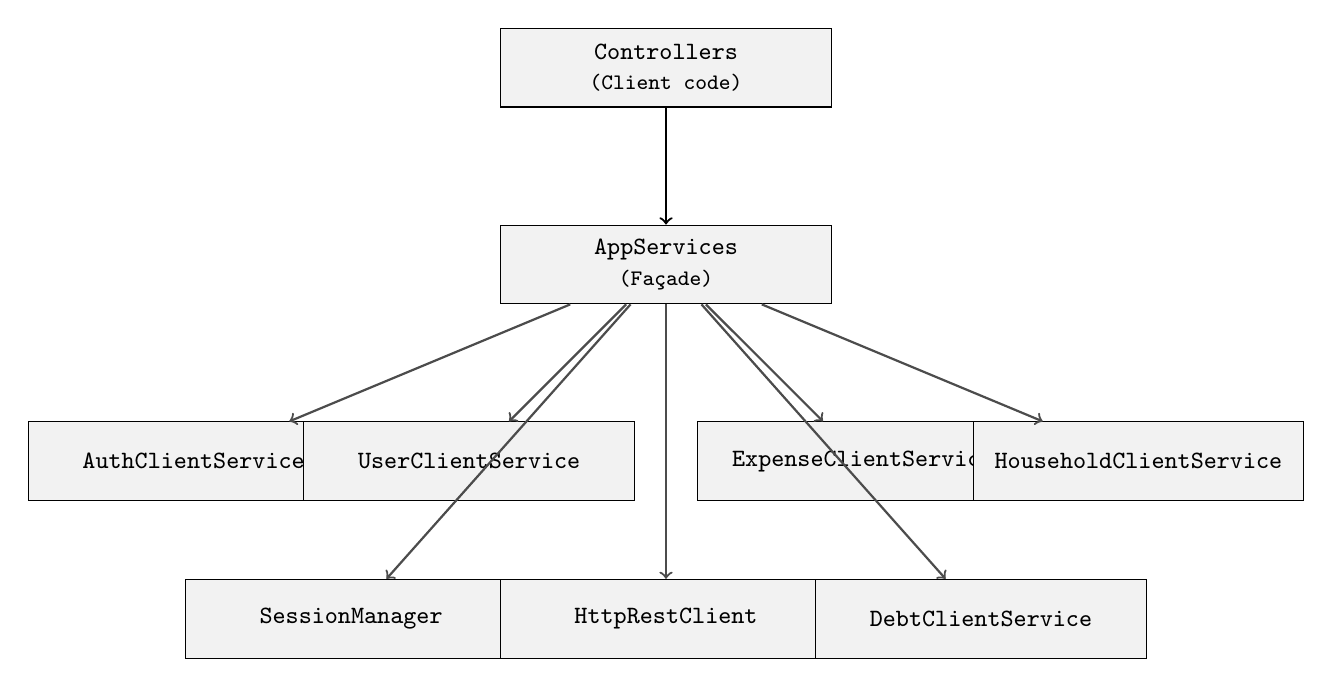
\begin{tikzpicture}[
    class/.style={
        rectangle, draw=black, fill=gray!10,
        minimum width=4.2cm, minimum height=1cm,
        align=center, font=\small\ttfamily
    },
    uses/.style={->, thick},
    contains/.style={->, thick, draw=black!70}
]

% Facade
\node[class] (facade) at (0, 3) {
    \textbf{AppServices} \\
    \footnotesize (Fa\c{c}ade)
};

% Subsystem services
\node[class] (auth) at (-6, 0.5) {\textbf{AuthClientService}};
\node[class] (user) at (-2.5, 0.5) {\textbf{UserClientService}};
\node[class] (expense) at (2.5, 0.5) {\textbf{ExpenseClientService}};
\node[class] (household) at (6, 0.5) {\textbf{HouseholdClientService}};
\node[class] (session) at (-4, -1.5) {\textbf{SessionManager}};
\node[class] (http) at (0, -1.5) {\textbf{HttpRestClient}};
\node[class] (debt) at (4, -1.5) {\textbf{DebtClientService}};

% Client
\node[class] (client) at (0, 5.5) {
    \textbf{Controllers} \\
    \footnotesize (Client code)
};

% Relationships
\draw[uses] (client) -- (facade);
\draw[contains] (facade) -- (auth);
\draw[contains] (facade) -- (user);
\draw[contains] (facade) -- (expense);
\draw[contains] (facade) -- (household);
\draw[contains] (facade) -- (session);
\draw[contains] (facade) -- (http);
\draw[contains] (facade) -- (debt);

\end{tikzpicture}}%
\caption{Fa\c{c}ade Pattern: Unified Service Access}
\end{figure}

\textbf{Implementation description.} The \texttt{AppServices} class acts as a Fa\c{c}ade over the entire client-side service subsystem. It aggregates instances of all eight client services (\texttt{AuthClientService}, \texttt{UserClientService}, \texttt{HouseholdClientService}, \texttt{ChoreClientService}, \texttt{ExpenseClientService}, \texttt{DebtClientService}, \texttt{SettlementClientService}, \texttt{ShoppingListClientService}), the \texttt{SessionManager}, and the underlying \texttt{HttpRestClient}. Controllers never instantiate or manage service dependencies themselves; they receive a single \texttt{AppServices} reference during FXML loading and use its getters to access any service they need.

\textbf{Comparison with the standard.}
\begin{itemize}
    \item \textbf{Simplified interface:} The GoF Fa\c{c}ade pattern provides a unified, simplified interface to a complex subsystem. \texttt{AppServices} fulfills this precisely: without it, every controller would need to receive and manage references to eight independent services plus the session manager, resulting in extensive boilerplate code in each controller's constructor.
    \item \textbf{Not hiding the subsystem:} In the strict GoF definition, the Fa\c{c}ade can optionally hide the subsystem classes entirely, exposing only high-level methods. Our implementation exposes the individual services through getters (e.g., \texttt{getExpenseClientService()}) rather than wrapping their methods. This is a deliberate trade-off: wrapping every method of every service would create a monolithic class with dozens of delegating methods, contradicting the Single Responsibility Principle, while still providing no additional abstraction.
\end{itemize}

\subsection{Mediator Pattern}

\begin{figure}[H]
\centering
\resizebox{\textwidth}{!}{%
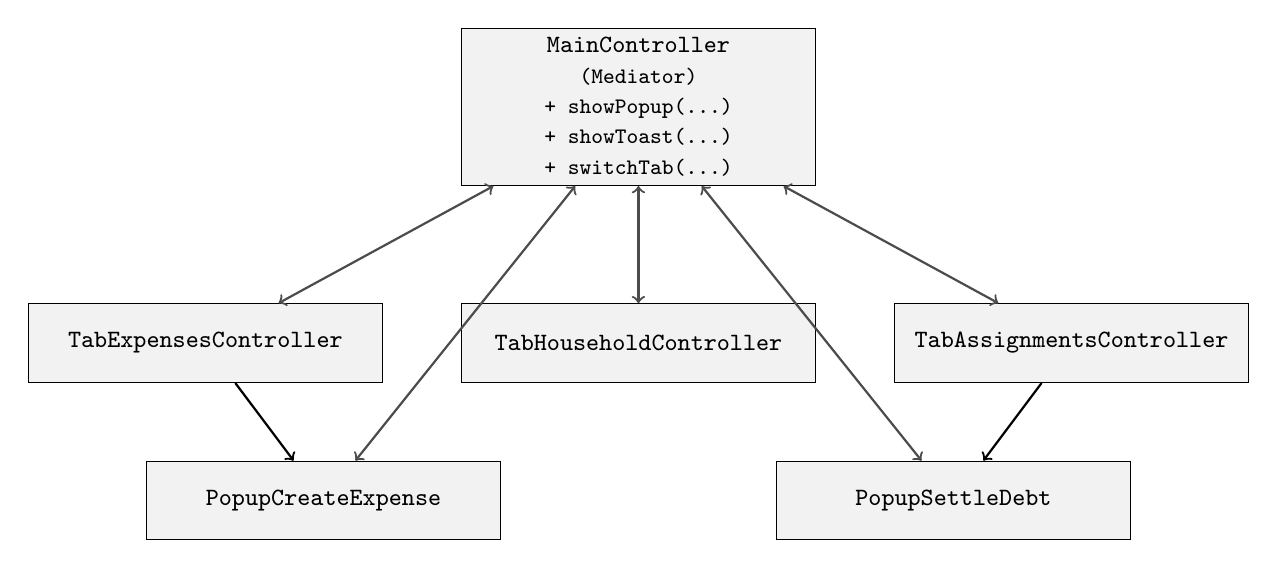
\begin{tikzpicture}[
    class/.style={
        rectangle, draw=black, fill=gray!10,
        minimum width=4.5cm, minimum height=1cm,
        align=center, font=\small\ttfamily
    },
    mediates/.style={<->, thick, draw=black!70},
    calls/.style={->, thick}
]

% Mediator
\node[class] (mediator) at (0, 3) {
    \textbf{MainController} \\
    \footnotesize (Mediator) \\
    \footnotesize + showPopup(...) \\
    \footnotesize + showToast(...) \\
    \footnotesize + switchTab(...)
};

% Colleagues
\node[class] (tab1) at (-5.5, 0) {\textbf{TabExpensesController}};
\node[class] (tab2) at (0, 0) {\textbf{TabHouseholdController}};
\node[class] (tab3) at (5.5, 0) {\textbf{TabAssignmentsController}};
\node[class] (popup1) at (-4, -2) {\textbf{PopupCreateExpense}};
\node[class] (popup2) at (4, -2) {\textbf{PopupSettleDebt}};

% Relationships
\draw[mediates] (tab1) -- (mediator);
\draw[mediates] (tab2) -- (mediator);
\draw[mediates] (tab3) -- (mediator);
\draw[calls] (tab1) -- (popup1);
\draw[calls] (tab3) -- (popup2);
\draw[mediates] (popup1) -- (mediator);
\draw[mediates] (popup2) -- (mediator);

\end{tikzpicture}}%
\caption{Mediator Pattern: Centralized UI Coordination}
\end{figure}

\textbf{Implementation description.} The \texttt{MainController} acts as a central Mediator for all user interface coordination in the JavaFX client. When the FXML hierarchy is loaded, every child controller (tabs and popups) receives a reference to the \texttt{MainController} via the \texttt{setControllerFactory} mechanism. Whenever a child controller needs to open a popup, display a success or error toast, or trigger a tab switch, it calls a method on the \texttt{MainController} (e.g., \texttt{showPopup}, \texttt{showToast}). No child controller ever communicates directly with another child controller; all cross-component interactions are routed through the mediator.

\textbf{Comparison with the standard.}
\begin{itemize}
    \item \textbf{Concrete vs Abstract Mediator:} The GoF pattern defines the Mediator as an interface or abstract class, allowing multiple mediator implementations. Our application uses a single concrete \texttt{MainController} because the JavaFX client has exactly one main window with one coordination point. Introducing an abstract mediator would add unnecessary complexity without a realistic use case for substitution.
    \item \textbf{Bidirectional communication:} In the standard pattern, colleagues notify the mediator of events, and the mediator decides how to respond. Our implementation follows this closely: child controllers call the mediator's methods (upward direction), and the mediator manipulates the shared \texttt{StackPane} layers to display popups and toasts (downward direction). The child controllers never directly access the \texttt{popupLayer} or \texttt{confirmPopupLayer} nodes.
    \item \textbf{Decoupling benefit:} Without this mediator, each of the 15+ controllers would need references to every other controller it might interact with, creating a tightly coupled mesh of dependencies. The mediator reduces this to a star topology where each controller knows only the \texttt{MainController}.
\end{itemize}
